\documentclass[tikz,border=2pt]{standalone}
\usepackage[T1]{fontenc}
\usepackage[scaled]{helvet}
\renewcommand{\familydefault}{\sfdefault}
\usepackage{tikz}
\usepackage{pifont}
\usepackage{fontawesome}
\usetikzlibrary{external,calc,shapes.callouts,shapes.arrows}
\usetikzlibrary{arrows.meta,patterns,patterns.meta,shapes.arrows}
\usetikzlibrary{decorations.pathreplacing}
\usetikzlibrary{shapes,arrows,positioning,calc,patterns,overlay-beamer-styles}
\usepackage{tcolorbox}
\usepackage{pgfplots}
\tikzset{>=Latex,
    max width/.style args={#1}{
        execute at begin node={\begin{varwidth}{#1}},
        execute at end node={\end{varwidth}}
    }
}
\usetikzlibrary{shapes}
\usetikzlibrary{external}
\begin{document}
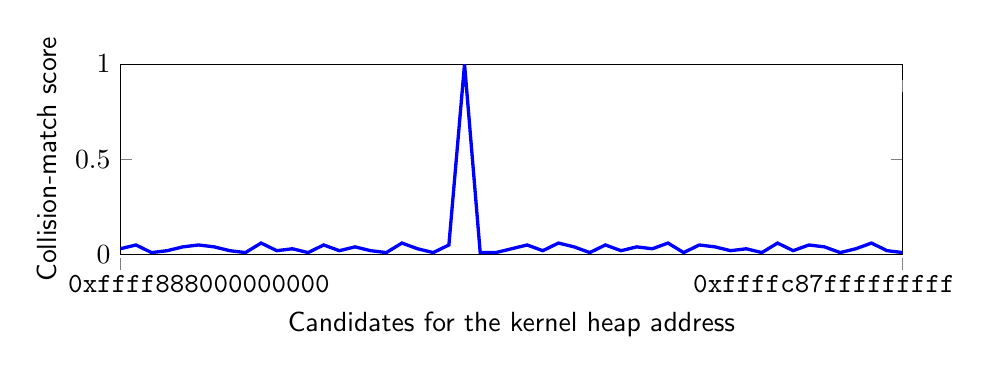
\begin{tikzpicture}
    \begin{axis}[
            width=0.95\textwidth,
            height=4cm,
            xmin=0,
            xmax=50,
            xtick={0},
            xticklabels={\texttt{0xffff888000000000}},
            extra x ticks={50},
            extra x tick labels={\texttt{0xffffc87fffffffff}},
            xlabel={Candidates for the kernel heap address},
            x tick style={yshift=-2mm},
            x tick label style={yshift=-1.5mm, xshift=1cm},
            extra x tick style={xticklabel style={xshift=-2cm}},
            ymin=0,
            ymax=1,
            ytick={0,0.5,1},
            ylabel={Collision-match score},
        ]

        \addplot[mark=None,color=blue,very thick] coordinates { (0,0.03) (1,0.05) (2,0.01) (3,0.02) (4,0.04) (5,0.05) (6,0.04) (7,0.02) (8,0.01) (9,0.06) (10,0.02) (11,0.03) (12,0.01) (13,0.05) (14,0.02) (15,0.04) (16,0.02) (17,0.01) (18,0.06) (19,0.03) (20,0.01) (21,0.05) (22,1) (23,0.01) (24,0.01) (25,0.03) (26,0.05) (27,0.02) (28,0.06) (29,0.04) (30,0.01) (31,0.05) (32,0.02) (33,0.04) (34,0.03) (35,0.06) (36,0.01) (37,0.05) (38,0.04) (39,0.02) (40,0.03) (41,0.01) (42,0.06) (43,0.02) (44,0.05) (45,0.04) (46,0.01) (47,0.03) (48,0.06) (49,0.02) (50,0.01)};
    \end{axis}
\end{tikzpicture}
\end{document}
